%!TEX root=../../root.tex

The vector projection of a vector $\mathbf{a}$ on (or onto) a nonzero vector $\mathbf{b}$ is the orthogonal projection of $\mathbf{a}$ onto a straight line parallel to $\mathbf{b}$. It is a vector parallel to $\mathbf{b}$, defined as: $\mathbf{a}_{1}=a_{1}\mathbf{\hat {b}}$, where $a_{1}$ is a scalar, called the scalar projection of $\mathbf{a}$ onto $\mathbf{b}$, and $\mathbf{\hat{b}}$ is the unit vector in the direction of $\mathbf{b}$. In turn, the scalar projection is defined as: $a_{1}=\left\|\mathbf {a} \right\|\cos \theta =\mathbf {a} \cdot \mathbf{\hat{b}} = {\frac {\mathbf {a \cdot b} }{\left\|\mathbf {b} \right\|}}\,$ where the operator $\cdot$ denotes a dot product, $\|\mathbf{a}\|$ is the length of $\mathbf{a}$, and $\theta$ is the angle between $\mathbf{a}$ and $\mathbf{b}$. The scalar projection is equal to the length of the vector projection, with a minus sign if the direction of the projection is opposite to the direction of $\mathbf{b}$. 

\begin{figure}[H]
	\centering
	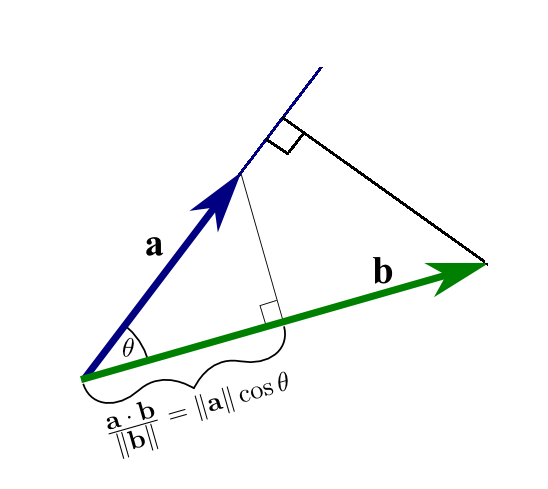
\includegraphics[width=.5\textwidth]{figures/A_proj.png}
	\caption{Projection of $\mathbf{a}$ on $\mathbf{b}$}\label{fig:A_proj}	
\end{figure}